\section{Experimental Results}
\label{sec:results}

We structure the experimental evidence around seven sequential research
questions that move from causal validation at $130\text{M}$ to design
ablation, full-budget tuning, multi-seed replication, horizon and parameter
scaling, contemporary two-sided baselines, and eight-GPU wall-clock efficiency:
\begin{enumerate}
\item[\textbf{Q1}] Does output-cotangent normalization improve loss beyond
  matched execution-path nulls, and is the mechanism directional rotation rather
  than step-size inflation? (Section~\ref{sec:res-q1})
\item[\textbf{Q2}] Why does asymmetric width-thresholding (\taxid{WT-MLP})
  outperform both full dense preconditioning (\taxid{DT-All}) and symmetric
  width-$4d$ diagonalization (\taxid{WT-Sym})? (Section~\ref{sec:res-q2})
\item[\textbf{Q3}] Does the advantage survive independent full-budget
  learning-rate tuning without short-horizon artifacts? (Section~\ref{sec:res-q3})
\item[\textbf{Q4}] Does the gain replicate across fresh post-selection seeds and
  16 external Paloma domains? (Section~\ref{sec:res-q4})
\item[\textbf{Q5}] Does \taxid{WT-MLP-Lag} persist under $4\times$ Chinchilla
  overtraining ($80$ TPP) and $4\times$ parameter scaling to $520\text{M}$
  ($799.6\text{M}$ total)? (Section~\ref{sec:res-q5})
\item[\textbf{Q6}] How does \taxid{WT-MLP} behave relative to contemporary
  two-sided Muon designs (Mousse and GO-MUON) under common isotropic decay?
  (Section~\ref{sec:res-q6})
\item[\textbf{Q7}] What is the executed eight-A100 latency, memory footprint,
  and wall-clock time-to-target under \texttt{fast\_lag}? (Section~\ref{sec:res-q7})
\end{enumerate}

\subsection{Q1: Complementarity, Causal Null Attribution, and Step-Norm Invariance}
\label{sec:res-q1}

\paragraph{Output-cotangent whitening complements input whitening and fails when substituted for it.}
Applying identical dense output factors to all 224 block matrices improves
11-point late selection loss by $-0.0058$ nats when added on top of input
whitening (\taxid{DT-All} in Table~\ref{tab:main}), but degrades loss by
$+0.0087$ nats when replacing input whitening (\taxid{Abl-OutOnly}) --- a
$0.0145$-nat swing between two arms with identical left factors. The same
asymmetry holds when restricted to the 32 down-projection matrices
(\taxid{Abl-DownOnly} at $-0.0014$ versus \taxid{Abl-DownSwap} at $+0.0025$),
and diagonalizing width-$512$ inputs alongside outputs (\taxid{Abl-BothDiag})
produces the worst regression in the study ($+0.0180$ nats, worse than plain
\taxid{Muon} at $+0.0055$). Input whitening conditions the domain entering
$\Nten$; output whitening provides distinct codomain information that cannot
substitute for it.

\paragraph{Matched execution-path nulls absorb legacy runtime artifacts while confirming a robust net geometry gain.}
Running the full output capture, reduction, and root pipeline with identity left
factors ($L = \hat L = I$) reveals non-zero execution-path drift on the legacy
runner: \taxid{Null-Dense} improves selection loss by $-0.0013$ nats ($22\%$ of
\taxid{DT-All}'s raw gain) and C4 by $-0.0023$ nats, while legacy Wave-3
\taxid{Null-WT} improves selection by $-0.0006$ and C4 by $-0.0020$ nats
(Figure~\ref{fig:q1}a). Subtracting each family's matched null still leaves
$-0.0059$ selection and $-0.0040$ C4 nats of net geometry gain for
\taxid{WT-MLP} (and $-0.0045$ selection / $-0.0041$ C4 for \taxid{DT-All}),
whereas weak outer-only variants (\taxid{Abl-DownOnly} at $-0.0001$ net;
\taxid{OD-Outer} at $-0.0004$ net) collapse to noise once the null is
subtracted. On the unified \texttt{fast\_lag} runner (Phase~1 of
Table~\ref{tab:confirmation}), the \taxid{Null-WT} artifact shrinks nearly
threefold to $\confNullFinalSelDelta{}$ final ($\confNullLateSelDelta{}$
late-11) selection and $\confNullLateCfourDelta{}$ late-11 C4, preserving
$\confPOneZeroTwoTwoWtNetLateSel{}$ late-11 ($\confPOneZeroTwoTwoWtNetFinalSel{}$
final) net selection gain for \taxid{WT-MLP-Lag}.

\paragraph{Output preconditioning improves loss by rotating updates at matched Frobenius norm rather than inflating effective step size.}
Evaluating two-sided direction $D = \hat L \Nten(L U R)\hat R$ against
input-only $D_{\text{in}} = \Nten(U R)\hat R$ on identical pre-update states
$(U, R, \hat R)$ across all 224 matrices at update $2{,}500$ rules out implicit
step-size inflation: the Frobenius norm ratio $\|D\|_F / \|D_{\text{in}}\|_F$ is
$\mechMlpdiagGraftNorm{}$ for \taxid{WT-MLP}, $\mechLeftdiagGraftNorm{}$ for
\taxid{OD-All}, and $\mechDenseGraftNorm{}$ for \taxid{DT-All} (and
$\mechMlpdiagEndGraftNorm{}$ for \taxid{WT-MLP} at update $5{,}120$, with final
block weight norm $\mechMlpdiagWeightDiffEndPct\%$ smaller than \taxid{MuonT}).
At this matched norm, \taxid{WT-MLP} rotates updates by a mean of
$\mechMlpdiagGraftDeg^\circ$ across all seven projections
(Figure~\ref{fig:q1}b), whereas \taxid{OD-All}'s rotation collapses to
$\mechLeftdiagOutODeg^\circ$ on \texttt{o} and $\mechLeftdiagOutDownDeg^\circ$
on \texttt{down} (versus $\mechMlpdiagOutODeg^\circ$ and
$\mechMlpdiagOutDownDeg^\circ$ in \taxid{WT-MLP}), mirroring
Table~\ref{tab:motivation}'s $1.2\%$ diagonal fidelity on residual-stream
cotangents.

\begin{table}[t]
\centering
\caption{Core seed-0 geometry ablations, matched execution-path nulls, and
matched eight-A100 costs across all six taxonomic families ($130\text{M}$
$1\times$ Chinchilla, $2.68\text{B}$ tokens, $\eta=0.0226$ except \taxid{Muon}
at $0.016$; negative loss deltas favor the candidate). \textbf{Raw $\Delta$Sel}
and \textbf{$\Delta$C4} average the 11 second-half evaluations
($\text{step} > 2{,}560$); \textbf{$\Delta$Train $\pm$ SE} is the
autocorrelation-inflated paired per-update training difference over the final
$1{,}024$ updates ($536.9\text{M}$ tokens). \textbf{Net $\Delta$Sel} subtracts
each family's matched null (\taxid{Null-WT}, \taxid{Null-Dense}, or same-wave
\taxid{Null-OD} ${}^{\dagger}$; ${}^{\S}$ uses conservative \taxid{Null-Dense}).
Rows marked ${}^{\ddagger}$ are executed on uncontended \texttt{fast\_lag}
nodes paired against same-wave \taxid{MuonT}. \textbf{Mean Step \%} and
\textbf{Peak GiB} come from the unified 96-update \texttt{bench\_8gpu\_opt}
benchmark (mean of updates 37--96 relative to \taxid{MuonT}; full-run timings
appear in Tables~\ref{tab:confirmation} and~\ref{tab:systems-v2}).}
\label{tab:main}
\scriptsize\setlength{\tabcolsep}{3.8pt}
\resizebox{\textwidth}{!}{% Generated by scripts/render_results_viz.py. Costs: results/measured_8gpu_timings.json. Do not edit.
\begin{tabular}{@{}lcrrrrrr@{}}
\toprule
Arm (\texttt{key}) & $\mathcal{A}(R_{512},R_{2048}\mid L_{512},L_{2048}\mid\tau)$ & Raw $\Delta$Sel & Net $\Delta$Sel & $\Delta$C4 & $\Delta$Train $\pm$ SE & Mean Step \% & Peak GiB \\
\midrule
\multicolumn{8}{@{}l}{\textcolor{famRef}{\pagesfsb I.\ Baselines (\texttt{Ref})}} \\
\taxid{MuonT} {\scriptsize(\muont{})} & \tcfg{\fFull}{\fFull}{\fNone}{\fNone}{0} & $0.0000$ & $0.0000$ & $0.0000$ & $0.0000 \pm \text{---}$ & $0.0$ & $20.5$ \\
\taxid{Muon} {\scriptsize(\texttt{muon})} & \tcfg{\fNone}{\fNone}{\fNone}{\fNone}{\text{---}} & $+0.0055$ & --- & $+0.0053$ & $+0.0062 \pm .00016$ & $-5.9$ & $19.0$ \\
\addlinespace[2.5pt]
\multicolumn{8}{@{}l}{\textcolor{famWT}{\pagesfsb II.\ Width-Thresholded Two-Sided (\texttt{WT} --- Asymmetric \& Symmetric $2\times 2$ Factorial)}} \\
\rowcolor{pagepanel} \textbf{\taxid{WT-MLP}} {\scriptsize(\texttt{mlpdiag})} & \tcfg{\fFull}{\fFull}{\fFull}{\fDiag}{0} & $\mathbf{-0.0066}$ & $\mathbf{-0.0059}$ & $-0.0061$ & $-0.0051 \pm .00004$ & $+14.7$ & $21.5$ \\
\rowcolor{pagepanel} \textbf{\taxid{WT-MLP-Lag}} {\scriptsize(\texttt{mlpdiag\_lag}, W4)} & \tcfg{\fFull}{\fFull}{\fFull}{\fDiag}{1} & $-0.0057$ & $\mathbf{-0.0050}$ & $-0.0050$ & $-0.0050 \pm .00004$ & $+10.7$ & $21.6$ \\
\rowcolor{pagepanel} \textbf{\taxid{WT-MLP-Lag}}$^{\ddagger}$ {\scriptsize(\texttt{fast\_lag})} & \tcfg{\fFull}{\fFull}{\fFull}{\fDiag}{1} & $-0.0047$ & $\mathbf{-0.0041}^{\ddagger}$ & $-0.0026$ & $-0.0020 \pm .00004$ & $+10.7$ & $21.6$ \\
\rowcolor{pagepanel} \textbf{\taxid{WT-Sym}}$^{\ddagger}$ {\scriptsize(\texttt{sym\_mlpdiag})} & \tcfg{\fFull}{\fDiag}{\fFull}{\fDiag}{0} & $-0.0025$ & $-0.0019^{\ddagger}$ & $-0.0020$ & $-0.0013 \pm .00005$ & $+8.6$ & $20.7$ \\
\rowcolor{pagepanel} \textbf{\taxid{WT-Sym-Lag}}$^{\ddagger}$ {\scriptsize(\texttt{sym\_mlpdiag\_lag})} & \tcfg{\fFull}{\fDiag}{\fFull}{\fDiag}{1} & $-0.0011$ & $-0.0005^{\ddagger}$ & $-0.0016$ & $-0.0015 \pm .00004$ & $+3.1$ & $20.8$ \\
\addlinespace[2.5pt]
\multicolumn{8}{@{}l}{\textcolor{famOD}{\pagesfsb III.\ Pure-Diagonal Output (\texttt{OD} --- Zero-Eigendecomposition Limit)}} \\
\rowcolor{pagepanel} \textbf{\taxid{OD-All}} {\scriptsize(\texttt{leftdiag})} & \tcfg{\fFull}{\fFull}{\fDiag}{\fDiag}{0} & $-0.0045$ & $-0.0032^{\S}$ & $-0.0036$ & $-0.0037 \pm .00004$ & $+1.3$ & $20.5$ \\
\taxid{OD-Outer}$^{\dagger}$ {\scriptsize(\texttt{outer\_leftdiag\_uf})} & \tcfg{\fFull}{\fFull}{\fOuterDiag}{\fOuterDiag}{0} & $-0.0025$ & $-0.0004$ & $-0.0026$ & $-0.0014 \pm .00005$ & $+1.4$ & $20.5$ \\
\addlinespace[2.5pt]
\multicolumn{8}{@{}l}{\textcolor{famDT}{\pagesfsb IV.\ Dense Two-Sided Ceiling (\texttt{DT})}} \\
\taxid{DT-All-Lag} {\scriptsize(\texttt{all\_lag})} & \tcfg{\fFull}{\fFull}{\fFull}{\fFull}{1} & $-0.0059$ & $-0.0046$ & $-0.0059$ & $-0.0057 \pm .00004$ & $+27.5$ & $24.8$ \\
\taxid{DT-All} {\scriptsize(\texttt{inner\_outer\_all})} & \tcfg{\fFull}{\fFull}{\fFull}{\fFull}{0} & $-0.0058$ & $-0.0045$ & $-0.0064$ & $-0.0050 \pm .00004$ & $+26.0$ & $24.2$ \\
\addlinespace[2.5pt]
\multicolumn{8}{@{}l}{\textcolor{famNull}{\pagesfsb V.\ Matched Execution-Path Nulls (\texttt{Null} --- Identity Left Factors)}} \\
\taxid{Null-WT} {\scriptsize(\texttt{null\_mlpdiag})} & \tcfg{\fFull}{\fFull}{\fNullFull}{\fNullDiag}{0} & $-0.0006$ & $0.0000$ & $-0.0020$ & $-0.0007 \pm .00004$ & $+15.0$ & $21.5$ \\
\taxid{Null-Dense} {\scriptsize(\texttt{null\_all})} & \tcfg{\fFull}{\fFull}{\fNullFull}{\fNullFull}{0} & $-0.0013$ & $0.0000$ & $-0.0023$ & $-0.0014 \pm .00004$ & $+32.3$ & $24.2$ \\
\taxid{Null-OD}$^{\dagger}$ {\scriptsize(\texttt{null\_leftdiag\_uf})} & \tcfg{\fFull}{\fFull}{\fNullDiag}{\fNullDiag}{0} & $-0.0020$ & $0.0000$ & $-0.0012$ & $-0.0011 \pm .00005$ & $+1.7$ & $20.5$ \\
\addlinespace[2.5pt]
\multicolumn{8}{@{}l}{\textcolor{famAbl}{\pagesfsb VI.\ Structural \& Input-Degradation Ablations (\texttt{Abl})}} \\
\taxid{Abl-OuterDense} {\scriptsize(\texttt{outer\_left\_all})} & \tcfg{\fFull}{\fFull}{\fOuterFull}{\fOuterFull}{0} & $-0.0040$ & $-0.0027$ & $-0.0048$ & $-0.0039 \pm .00004$ & $+25.6$ & $24.2$ \\
\taxid{Abl-No2048} {\scriptsize(\texttt{hidden})} & \tcfg{\fFull}{\fFull}{\fFull}{\fNone}{0} & $-0.0031$ & $-0.0024$ & $-0.0026$ & $-0.0021 \pm .00004$ & $+14.5$ & $21.5$ \\
\taxid{Abl-DownOnly} {\scriptsize(\texttt{outer\_left\_dn})} & \tcfg{\fFull}{\fFull}{\fOuterFull^{\text{dn}}}{\fNone}{0} & $-0.0014$ & $-0.0001^{\S}$ & $-0.0008$ & $-0.0012 \pm .00004$ & $+1.6$ & $20.8$ \\
\taxid{Abl-DownSwap} {\scriptsize(\texttt{down\_hybrid})} & \tcfg{\fFull}{\fNone}{\fFull^{\text{dn}}}{\fNone}{0} & $+0.0025$ & --- & $+0.0036$ & $+0.0032 \pm .00005$ & $-4.3$ & $19.4$ \\
\taxid{Abl-OutOnly} {\scriptsize(\texttt{left\_all})} & \tcfg{\fNone}{\fNone}{\fFull}{\fFull}{0} & $+0.0087$ & --- & $+0.0109$ & $+0.0079 \pm .00012$ & $+32.3$ & $22.2$ \\
\taxid{Abl-BothDiag} {\scriptsize(\texttt{all\_diag})} & \tcfg{\fDiag}{\fDiag}{\fDiag}{\fDiag}{0} & $+0.0180$ & --- & $+0.0177$ & $+0.0134 \pm .00031$ & $-4.6$ & $19.6$ \\
\bottomrule
\end{tabular}
}
\end{table}

\begin{figure}[t]
\centering
\resizebox{\textwidth}{!}{%
\begin{tikzpicture}
\begin{groupplot}[
  paperplot,
  group style={group size=2 by 1, horizontal sep=2.2cm},
  height=6.8cm,
]
\nextgroupplot[
  width=7.5cm,
  title={(a) Multi-metric causal attribution vs.\ \taxid{MuonT}},
  xlabel={$\Delta$ Loss versus \taxid{MuonT} (nats; left is better)},
  xmin=-0.0078, xmax=0.0118,
  ymin=-0.65, ymax=15.65,
  scaled x ticks=false,
  xtick={-0.006,-0.003,0,0.003,0.006,0.009},
  xticklabel style={/pgf/number format/fixed, /pgf/number format/precision=3, font=\tiny},
  ytick={0,1,2,3,4,5,6,7,8,9,10,11,12,13,14,15},
  yticklabels={
    {\taxid{Abl-BothDiag}},{\taxid{Abl-OutOnly}},{\taxid{Muon}},
    {\taxid{Abl-DownSwap}},{\taxid{Abl-DownOnly}},{\taxid{WT-Sym-Lag}$^{\ddagger}$},
    {\taxid{WT-Sym}$^{\ddagger}$},{\taxid{OD-Outer}$^{\dagger}$},{\taxid{Abl-No2048}},
    {\taxid{Abl-OuterDense}},{\textbf{\taxid{OD-All}}},{\taxid{DT-All}},
    {\taxid{DT-All-Lag}},{\textbf{\taxid{WT-MLP-Lag}}$^{\ddagger}$},
    {\taxid{WT-MLP-Lag} (W4)},{\textbf{\taxid{WT-MLP}}}
  },
  yticklabel style={font=\tiny},
  legend columns=2,
  legend style={at={(0.5,-0.17)}, anchor=north, font=\tiny, column sep=4pt},
]
% Generated by scripts/render_results_viz.py. Do not edit.
\fill[famWT!5] (axis cs:-0.0078,3.52) rectangle (axis cs:0.0,15.65);
\fill[famAbl!4] (axis cs:0.0,-0.65) rectangle (axis cs:0.0118,3.52);
\draw[pagemuted!75, line width=0.6pt] (axis cs:0,-0.65) -- (axis cs:0,15.65);
\draw[pagemuted!65, densely dashed, line width=0.55pt] (axis cs:-0.0078,3.52) -- (axis cs:0.0118,3.52);
\node[font=\tiny\itshape, text=pagemuted!95!black, anchor=south east] at (axis cs:0.0115,3.72) {Two-sided additions ($\uparrow$)};
\node[font=\tiny\itshape, text=famAbl!85!black, anchor=north west, align=left] at (axis cs:-0.0075,3.34) {Input removed /\\ degraded ($\downarrow$)};
\addplot[area legend, fill=famNull!42, draw=famNull!85] coordinates {(1,-10) (1,-10)};
\addlegendentry{Null path share}
\addplot[area legend, fill=famWT!75, draw=famWT!95] coordinates {(1,-10) (1,-10)};
\addlegendentry{Net geometry $\Delta$Sel}
\addplot[only marks, mark=diamond*, mark size=2.1pt, mark options={fill=white, draw=pageink, line width=0.65pt}] coordinates {(1,-10)};
\addlegendentry{$\Delta$C4}
\addplot[only marks, mark=*, mark size=1.4pt, color=pageink] coordinates {(1,-10)};
\addlegendentry{Paired $\Delta$Train ($\pm 2\,\mathrm{SE}$)}
\filldraw[fill=famNull!42, draw=famNull!85, line width=0.45pt] (axis cs:0,14.76) rectangle (axis cs:-0.000649,15.24);
\filldraw[fill=famWT!76, draw=famWT!95, line width=0.5pt] (axis cs:-0.000649,14.76) rectangle (axis cs:-0.006584,15.24);
\draw[pageink, line width=0.65pt] (axis cs:-0.005155,15) -- (axis cs:-0.004975,15);
\draw[pageink, line width=0.55pt] (axis cs:-0.005155,14.89) -- (axis cs:-0.005155,15.11);
\draw[pageink, line width=0.55pt] (axis cs:-0.004975,14.89) -- (axis cs:-0.004975,15.11);
\filldraw[fill=famNull!42, draw=famNull!85, line width=0.45pt] (axis cs:0,13.76) rectangle (axis cs:-0.000649,14.24);
\filldraw[fill=famWT!76, draw=famWT!95, line width=0.5pt] (axis cs:-0.000649,13.76) rectangle (axis cs:-0.005683,14.24);
\draw[pageink, line width=0.65pt] (axis cs:-0.005034,14) -- (axis cs:-0.004869,14);
\draw[pageink, line width=0.55pt] (axis cs:-0.005034,13.89) -- (axis cs:-0.005034,14.11);
\draw[pageink, line width=0.55pt] (axis cs:-0.004869,13.89) -- (axis cs:-0.004869,14.11);
\filldraw[fill=famNull!42, draw=famNull!85, line width=0.45pt] (axis cs:0,12.76) rectangle (axis cs:-0.000649,13.24);
\filldraw[fill=famWT!76, draw=famWT!95, line width=0.5pt] (axis cs:-0.000649,12.76) rectangle (axis cs:-0.004737,13.24);
\draw[pageink, line width=0.65pt] (axis cs:-0.002077,13) -- (axis cs:-0.001916,13);
\draw[pageink, line width=0.55pt] (axis cs:-0.002077,12.89) -- (axis cs:-0.002077,13.11);
\draw[pageink, line width=0.55pt] (axis cs:-0.001916,12.89) -- (axis cs:-0.001916,13.11);
\filldraw[fill=famNull!42, draw=famNull!85, line width=0.45pt] (axis cs:0,11.76) rectangle (axis cs:-0.001286,12.24);
\filldraw[fill=famDT!76, draw=famDT!95, line width=0.5pt] (axis cs:-0.001286,11.76) rectangle (axis cs:-0.005893,12.24);
\draw[pageink, line width=0.65pt] (axis cs:-0.005811,12) -- (axis cs:-0.005647,12);
\draw[pageink, line width=0.55pt] (axis cs:-0.005811,11.89) -- (axis cs:-0.005811,12.11);
\draw[pageink, line width=0.55pt] (axis cs:-0.005647,11.89) -- (axis cs:-0.005647,12.11);
\filldraw[fill=famNull!42, draw=famNull!85, line width=0.45pt] (axis cs:0,10.76) rectangle (axis cs:-0.001286,11.24);
\filldraw[fill=famDT!76, draw=famDT!95, line width=0.5pt] (axis cs:-0.001286,10.76) rectangle (axis cs:-0.005782,11.24);
\draw[pageink, line width=0.65pt] (axis cs:-0.005055,11) -- (axis cs:-0.004895,11);
\draw[pageink, line width=0.55pt] (axis cs:-0.005055,10.89) -- (axis cs:-0.005055,11.11);
\draw[pageink, line width=0.55pt] (axis cs:-0.004895,10.89) -- (axis cs:-0.004895,11.11);
\filldraw[fill=famNull!42, draw=famNull!85, line width=0.45pt] (axis cs:0,9.76) rectangle (axis cs:-0.001286,10.24);
\filldraw[fill=famOD!76, draw=famOD!95, line width=0.5pt] (axis cs:-0.001286,9.76) rectangle (axis cs:-0.004503,10.24);
\draw[pageink, line width=0.65pt] (axis cs:-0.003772,10) -- (axis cs:-0.003603,10);
\draw[pageink, line width=0.55pt] (axis cs:-0.003772,9.89) -- (axis cs:-0.003772,10.11);
\draw[pageink, line width=0.55pt] (axis cs:-0.003603,9.89) -- (axis cs:-0.003603,10.11);
\filldraw[fill=famNull!42, draw=famNull!85, line width=0.45pt] (axis cs:0,8.76) rectangle (axis cs:-0.001286,9.24);
\filldraw[fill=famAbl!76, draw=famAbl!95, line width=0.5pt] (axis cs:-0.001286,8.76) rectangle (axis cs:-0.003977,9.24);
\draw[pageink, line width=0.65pt] (axis cs:-0.003960,9) -- (axis cs:-0.003795,9);
\draw[pageink, line width=0.55pt] (axis cs:-0.003960,8.89) -- (axis cs:-0.003960,9.11);
\draw[pageink, line width=0.55pt] (axis cs:-0.003795,8.89) -- (axis cs:-0.003795,9.11);
\filldraw[fill=famNull!42, draw=famNull!85, line width=0.45pt] (axis cs:0,7.76) rectangle (axis cs:-0.000649,8.24);
\filldraw[fill=famAbl!76, draw=famAbl!95, line width=0.5pt] (axis cs:-0.000649,7.76) rectangle (axis cs:-0.003068,8.24);
\draw[pageink, line width=0.65pt] (axis cs:-0.002209,8) -- (axis cs:-0.002054,8);
\draw[pageink, line width=0.55pt] (axis cs:-0.002209,7.89) -- (axis cs:-0.002209,8.11);
\draw[pageink, line width=0.55pt] (axis cs:-0.002054,7.89) -- (axis cs:-0.002054,8.11);
\filldraw[fill=famNull!42, draw=famNull!85, line width=0.45pt] (axis cs:0,6.76) rectangle (axis cs:-0.002010,7.24);
\filldraw[fill=famOD!76, draw=famOD!95, line width=0.5pt] (axis cs:-0.002010,6.76) rectangle (axis cs:-0.002453,7.24);
\draw[pageink, line width=0.65pt] (axis cs:-0.001469,7) -- (axis cs:-0.001287,7);
\draw[pageink, line width=0.55pt] (axis cs:-0.001469,6.89) -- (axis cs:-0.001469,7.11);
\draw[pageink, line width=0.55pt] (axis cs:-0.001287,6.89) -- (axis cs:-0.001287,7.11);
\filldraw[fill=famNull!42, draw=famNull!85, line width=0.45pt] (axis cs:0,5.76) rectangle (axis cs:-0.000649,6.24);
\filldraw[fill=famWT!76, draw=famWT!95, line width=0.5pt] (axis cs:-0.000649,5.76) rectangle (axis cs:-0.002515,6.24);
\draw[pageink, line width=0.65pt] (axis cs:-0.001352,6) -- (axis cs:-0.001171,6);
\draw[pageink, line width=0.55pt] (axis cs:-0.001352,5.89) -- (axis cs:-0.001352,6.11);
\draw[pageink, line width=0.55pt] (axis cs:-0.001171,5.89) -- (axis cs:-0.001171,6.11);
\filldraw[fill=famNull!42, draw=famNull!85, line width=0.45pt] (axis cs:0,4.76) rectangle (axis cs:-0.000649,5.24);
\filldraw[fill=famWT!76, draw=famWT!95, line width=0.5pt] (axis cs:-0.000649,4.76) rectangle (axis cs:-0.001127,5.24);
\draw[pageink, line width=0.65pt] (axis cs:-0.001558,5) -- (axis cs:-0.001397,5);
\draw[pageink, line width=0.55pt] (axis cs:-0.001558,4.89) -- (axis cs:-0.001558,5.11);
\draw[pageink, line width=0.55pt] (axis cs:-0.001397,4.89) -- (axis cs:-0.001397,5.11);
\filldraw[fill=famNull!42, draw=famNull!85, line width=0.45pt] (axis cs:0,3.76) rectangle (axis cs:-0.001286,4.24);
\filldraw[fill=famAbl!76, draw=famAbl!95, line width=0.5pt] (axis cs:-0.001286,3.76) rectangle (axis cs:-0.001370,4.24);
\draw[pageink, line width=0.65pt] (axis cs:-0.001239,4) -- (axis cs:-0.001081,4);
\draw[pageink, line width=0.55pt] (axis cs:-0.001239,3.89) -- (axis cs:-0.001239,4.11);
\draw[pageink, line width=0.55pt] (axis cs:-0.001081,3.89) -- (axis cs:-0.001081,4.11);
\filldraw[fill=famAbl!48, draw=famAbl!88, line width=0.5pt] (axis cs:0,2.76) rectangle (axis cs:0.002512,3.24);
\draw[pageink, line width=0.65pt] (axis cs:0.003082,3) -- (axis cs:0.003270,3);
\draw[pageink, line width=0.55pt] (axis cs:0.003082,2.89) -- (axis cs:0.003082,3.11);
\draw[pageink, line width=0.55pt] (axis cs:0.003270,2.89) -- (axis cs:0.003270,3.11);
\filldraw[fill=famRef!48, draw=famRef!88, line width=0.5pt] (axis cs:0,1.76) rectangle (axis cs:0.005505,2.24);
\draw[pageink, line width=0.65pt] (axis cs:0.005841,2) -- (axis cs:0.006481,2);
\draw[pageink, line width=0.55pt] (axis cs:0.005841,1.89) -- (axis cs:0.005841,2.11);
\draw[pageink, line width=0.55pt] (axis cs:0.006481,1.89) -- (axis cs:0.006481,2.11);
\filldraw[fill=famAbl!48, draw=famAbl!88, line width=0.5pt] (axis cs:0,0.76) rectangle (axis cs:0.008707,1.24);
\draw[pageink, line width=0.65pt] (axis cs:0.007636,1) -- (axis cs:0.008096,1);
\draw[pageink, line width=0.55pt] (axis cs:0.007636,0.89) -- (axis cs:0.007636,1.11);
\draw[pageink, line width=0.55pt] (axis cs:0.008096,0.89) -- (axis cs:0.008096,1.11);
\filldraw[fill=famAbl!48, draw=famAbl!88, line width=0.5pt] (axis cs:0,-0.24) rectangle (axis cs:0.011300,0.24);
\draw[-Latex, famAbl!95!black, line width=0.75pt] (axis cs:0.0104,0) -- (axis cs:0.01165,0);
\node[font=\tiny, text=famAbl!95!black, fill=white, fill opacity=0.88, text opacity=1, anchor=east, inner sep=1pt] at (axis cs:0.0103,0) {$+0.0180$};
\addplot[only marks, forget plot, mark=diamond*, mark size=2.0pt, mark options={fill=white, draw=pageink, line width=0.65pt}] coordinates {(-0.006078,15) (-0.004987,14) (-0.002621,13) (-0.005863,12) (-0.006379,11) (-0.003610,10) (-0.004774,9) (-0.002625,8) (-0.002597,7) (-0.002028,6) (-0.001603,5) (-0.000782,4) (0.003605,3) (0.005345,2) (0.010896,1)};
\addplot[only marks, forget plot, mark=*, mark size=1.3pt, color=pageink] coordinates {(-0.005065,15) (-0.004952,14) (-0.001996,13) (-0.005729,12) (-0.004975,11) (-0.003688,10) (-0.003877,9) (-0.002132,8) (-0.001378,7) (-0.001261,6) (-0.001478,5) (-0.001160,4) (0.003176,3) (0.006161,2) (0.007866,1)};


\nextgroupplot[
  width=7.2cm,
  ybar=1.6pt, bar width=6.5pt,
  title={(b) Update rotation at matched step norm (step 2{,}500)},
  xlabel={Block projection ($m\times n$)},
  ylabel={Rotation vs.\ $D_{\text{in}}$ (deg)},
  ymin=0, ymax=36.5,
  xmin=-0.55, xmax=6.55,
  xtick={0,1,2,3,4,5,6},
  xticklabels={\texttt{gate},\texttt{up},\texttt{q},\texttt{k},\texttt{v},\texttt{o},\texttt{down}},
  legend style={at={(0.98,0.97)}, anchor=north east, font=\tiny},
]
\addplot[fill=famWT!78, draw=famWT!95] table[x=idx, y=graft_deg_mlpdiag] {figs/mechanism_bars.dat};
\addlegendentry{\textbf{\taxid{WT-MLP}} (norm ratio $\mechMlpdiagGraftNorm$)}
\addplot[fill=famOD!75, draw=famOD!95] table[x=idx, y=graft_deg_leftdiag] {figs/mechanism_bars.dat};
\addlegendentry{\textbf{\taxid{OD-All}} (norm ratio $\mechLeftdiagGraftNorm$)}
\draw[famWT, densely dashed, line width=0.8pt] (axis cs:-0.55,\mechMlpdiagGraftDeg) -- (axis cs:6.55,\mechMlpdiagGraftDeg);
\node[font=\tiny, text=famWT!95!black, anchor=south west] at (axis cs:4.1,\mechMlpdiagGraftDeg) {mean $\mechMlpdiagGraftDeg^\circ$};
\end{groupplot}
\end{tikzpicture}%
}
\caption{Causal attribution and step-geometry verification at $130\text{M}$
($1\times$ Chinchilla, seed~0).
\textbf{(a)} Decomposition of raw 11-point late selection deltas into matched
execution-path null share (ochre) plus net geometry gain (family fill), overlaid
with external $\Delta\text{C4}$ diamonds and paired final-window
$\Delta\text{Train} \pm 2\,\text{SE}$ (above dashed divider: two-sided
candidates; below: input-degradation controls).
\textbf{(b)} Instantaneous angular rotation between two-sided update $D$ and
input-only $D_{\text{in}}$ on identical pre-update states across all 32 layers
at update $2{,}500$: both \taxid{WT-MLP} and \taxid{OD-All} match
\taxid{MuonT}'s Frobenius step norm within $1.5\%$, while diagonalizing
width-$512$ residual cotangents (\texttt{o}, \texttt{down}) collapses
\taxid{OD-All}'s rotation to $3.7^\circ$--$4.0^\circ$.}
\label{fig:q1}
\end{figure}

\subsection{Q2: Freshness vs.\ Richness and Asymmetric vs.\ Symmetric Width-\texorpdfstring{$4d$}{4d} Design}
\label{sec:res-q2}

\paragraph{Exact age-zero diagonal scale beats stale dense eigendecompositions on width-$4d$ pre-SwiGLU outputs.}
Replacing the two $2048\times 2048$ dense output roots (\texttt{out:gate},
\texttt{out:up}) with exact age-zero inline diagonals in \taxid{WT-MLP}
improves 11-point late selection loss \emph{past} the full-dense ceiling
\taxid{DT-All} ($-0.0066$ versus $-0.0058$ nats; $-0.0059$ versus $-0.0045$ net
of null), whereas omitting width-$2048$ output factors altogether
(\taxid{Abl-No2048}) captures less than half the gain ($-0.0031$ raw / $-0.0024$
net; Table~\ref{tab:main}). Run-level counters explain why
(Figure~\ref{fig:q2-freshness}): dense-output \taxid{DT-All} holds cached
eigenbases $\approx 3$ updates stale against a 4-update refresh target and
accumulates $31{,}759$ Rank-0 exact \texttt{eigh} fallbacks, whereas
\taxid{WT-MLP} cuts fallbacks by $\motFbMlpdiagDropPct\%$ (to
$\motFbRankZeroMlpdiagOut$) while tracking $82\%$--$88\%$ of pre-SwiGLU
anisotropy at age zero.

\paragraph{Symmetrically diagonalizing post-SwiGLU \texttt{in:down} (\taxid{WT-Sym}) incurs an early constant-LR penalty despite high diagonal root $R^2$.}
Although post-SwiGLU \texttt{in:down} shows high Frobenius inverse-square-root
fidelity ($R^2 = \motInDownExpVarLMedPct\%$ in Table~\ref{tab:motivation}),
extending diagonalization to \texttt{in:down} in the $2\times 2$ \texttt{fast\_lag}
comparison (\taxid{WT-Sym}, \taxid{WT-Sym-Lag}) imposes a
$\symLagVsMlpLagWinOne{} \pm \symLagVsMlpLagWinOneSe{}$-nat paired training-loss
penalty against \taxid{WT-MLP-Lag} across the 1{,}024-update constant-LR plateau
(Window~1; Figure~\ref{fig:q2-sym}). During linear LR decay, the gap narrows
monotonically ($\symLagVsMlpLagWinTwo{} \to \symLagVsMlpLagWinThree{} \to
\symLagVsMlpLagWinFour{} \to \symLagVsMlpLagWinFive{}$ across Windows~2--5),
reaching tied final C4 ($\symMlpLagCfourFinalAbs{}$ versus
$\fastMlpLagCfourFinalAbs{}$) while saving $\sysExecSymLagSavedMlpLagMs$\,ms/step
and $\sysExecSymLagSavedMlpLagGib$\,GiB; however, \taxid{WT-MLP-Lag} retains a
$\symLagVsMlpLagSelLateMag{}$-nat lead in 11-point late selection. Because
Frobenius root $R^2$ weights all matrix directions uniformly without accounting
for momentum alignment, \texttt{in:down}'s $56.6\%$ off-diagonal anisotropy
(and lower outer-root $R^2 = \motInDownExpVarLhatMedPct\%$), or input-shaped
decay $\lambda W \hat R^2$, asymmetric width-thresholding (\taxid{WT-MLP-Lag})
remains strictly superior for held-out mixture quality.

\begin{figure}[t]
\centering
\resizebox{\textwidth}{!}{%
\begin{tikzpicture}
\begin{groupplot}[
  paperplot,
  group style={group size=2 by 1, horizontal sep=2.15cm},
  width=7.35cm, height=4.7cm,
  every axis plot/.append style={line width=0.95pt},
]
\nextgroupplot[
  title={(a) Max output eigenbasis age in use},
  xlabel={Tokens processed (billions)}, ylabel={Max basis age (updates)},
  xmin=0, xmax=2.69, ymin=-0.2, ymax=5.1,
  legend style={at={(0.97,0.06)}, anchor=south east},
]
\addplot[color=famDT, densely dashed] table[x=tokens, y=inner_outer_all_age] {figs/freshness.dat};
\addlegendentry{\taxid{DT-All}}
\addplot[color=famWT, line width=1.1pt] table[x=tokens, y=inner_outer_mlpdiag_age] {figs/freshness.dat};
\addlegendentry{\textbf{\taxid{WT-MLP}}}
\addplot[color=famOD, line width=1.1pt] table[x=tokens, y=inner_outer_leftdiag_age] {figs/freshness.dat};
\addlegendentry{\taxid{OD-All}}

\nextgroupplot[
  title={(b) Cumulative Rank-0 exact \texttt{eigh} fallbacks},
  xlabel={Tokens processed (billions)}, ylabel={Cumulative fallbacks},
  xmin=0, xmax=2.69, ymin=0, ymax=34500,
  scaled y ticks=false, yticklabel style={/pgf/number format/fixed},
  legend style={at={(0.03,0.96)}, anchor=north west},
]
\addplot[color=famDT, densely dashed] table[x=tokens, y=inner_outer_all_fb] {figs/freshness.dat};
\addlegendentry{\taxid{DT-All} ($31{,}759$)}
\addplot[color=famWT, line width=1.1pt] table[x=tokens, y=inner_outer_mlpdiag_fb] {figs/freshness.dat};
\addlegendentry{\textbf{\taxid{WT-MLP}} ($\motFbRankZeroMlpdiagOut$)}
\addplot[color=famOD, line width=1.1pt] table[x=tokens, y=inner_outer_leftdiag_fb] {figs/freshness.dat};
\addlegendentry{\taxid{OD-All} ($0$)}
\end{groupplot}
\end{tikzpicture}%
}
\caption{Freshness versus staleness on $130\text{M}$ ($1\times$ Chinchilla,
seed~0; 64-update block means).
\textbf{(a)} Maximum output eigenbasis age in use: dense cached bases lag
roughly $3$ updates against a $4$-update refresh target, whereas inline
diagonals operate at age zero.
\textbf{(b)} Cumulative Rank-0 exact \texttt{cuSOLVER eigh} fallbacks:
diagonalizing width-$2048$ outputs in \taxid{WT-MLP} cuts fallbacks by
$\motFbMlpdiagDropPct\%$, and \taxid{OD-All} eliminates them completely.}
\label{fig:q2-freshness}
\end{figure}

\begin{figure}[t]
\centering
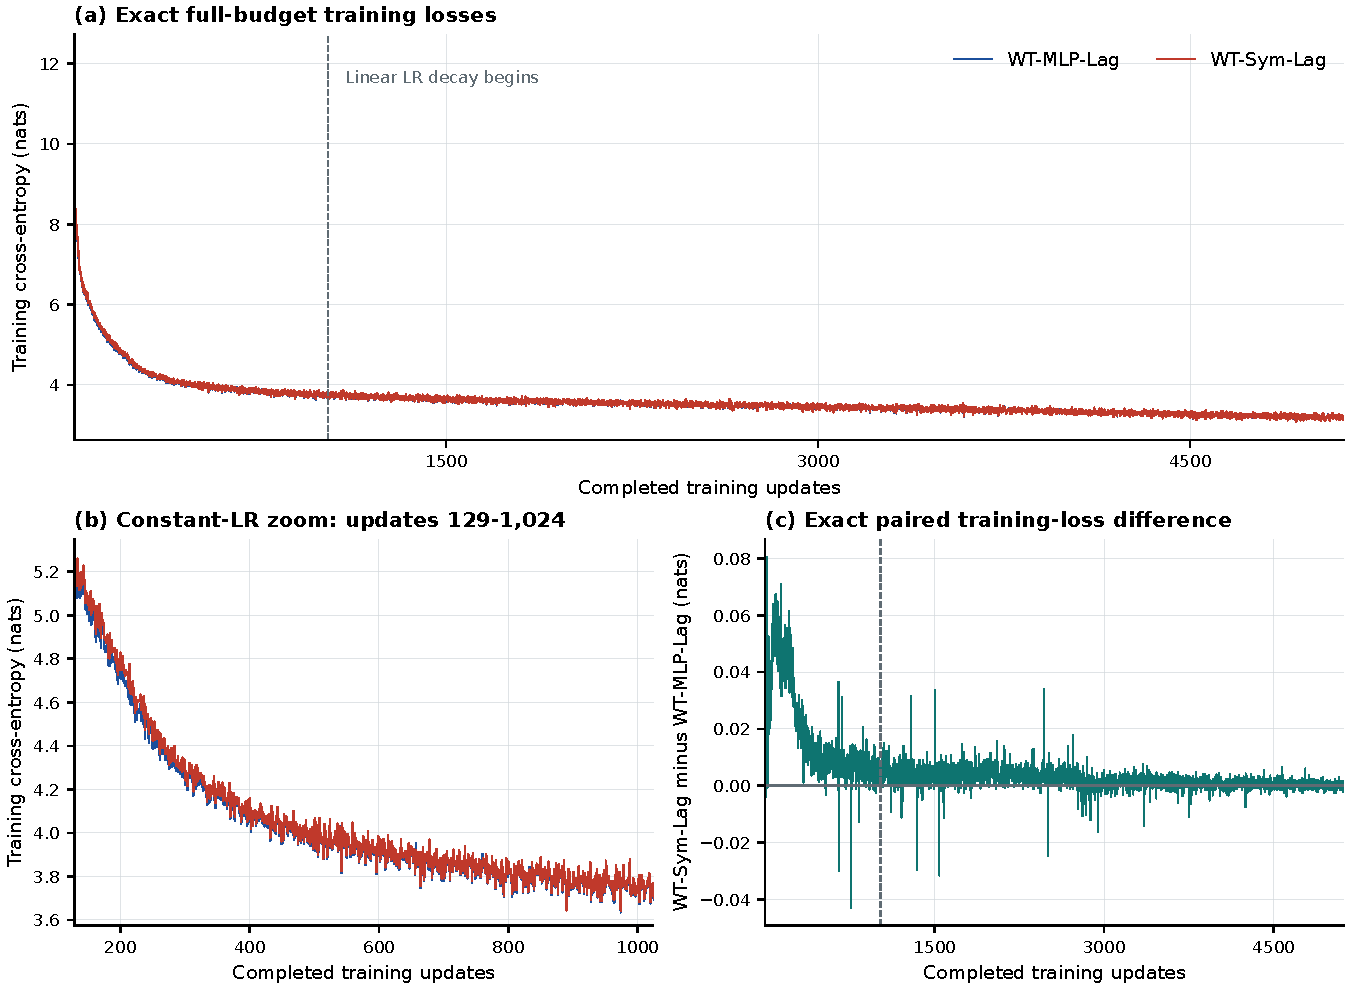
\includegraphics[width=\textwidth]{wt_lag_training.pdf}
\caption{Exact same-wave per-update training histories comparing asymmetric
\taxid{WT-MLP-Lag} against symmetric \taxid{WT-Sym-Lag} ($130\text{M}$ $1\times$,
seed~0, identical token order, \texttt{fast\_lag} runner; all $5{,}120$ logged
losses plotted with no smoothing, binning, or downsampling).
\textbf{(a)} Full $5{,}120$-update raw training loss per arm.
\textbf{(b)} Early constant-LR zoom over updates $129$--$1{,}024$.
\textbf{(c)} Exact paired difference (\taxid{WT-Sym-Lag} minus
\taxid{WT-MLP-Lag}; positive favors \taxid{WT-MLP-Lag}): diagonalizing
post-SwiGLU \texttt{in:down} incurs a $\symLagVsMlpLagWinOne{}$-nat mean
penalty during the constant-LR plateau (dashed vertical line at update
$1{,}024$) before contracting to $\symLagVsMlpLagWinFive{}$ during LR decay.}
\label{fig:q2-sym}
\end{figure}

\subsection{Q3: Learning-Rate Horizon Shift and Full-Budget LR Confirmation}
\label{sec:res-q3}

\paragraph{Short-schedule (320-step) learning-rate screening suffers severe horizon shift and invalidates transfer rankings.}
Before running full-budget tuning, we tested whether a 6\%-budget ($320$-update,
$0.17\text{B}$-token) seven-point sweep over $\eta \in [0.016, 0.128]$ could
predict full-budget optima (Figure~\ref{fig:q3}a). On the short schedule, every
arm shifted $2.8\times$--$4\times$ higher onto a flat plateau at $0.064$--$0.0905$,
where noise split two mathematically identical outer-diagonal arms
(\taxid{OD-Outer} versus \taxid{OD-Outer-F}) across $0.0905$ and $0.064$.
Carrying $0.064$ to the full 5{,}120-update budget \emph{degraded \taxid{MuonT}
itself by $\waveTwelveMuontSelDiff{}$ nats} relative to $0.0226$
($\waveTwelveMuontCfourDiff{}$ final C4), while pushing \taxid{OD-All} and
\taxid{OD-Outer} to $0.0905$ crossed the full-budget stability cliff
($+0.049$--$+0.050$ nats; Figure~\ref{fig:q3}b). Short-horizon screening is
therefore an invalid proxy; full-budget bracketing around $0.0226$ is mandatory.

\paragraph{Full-budget LR bracketing around $0.0226$ confirms that \taxid{WT-MLP-Lag} beats \taxid{MuonT} at every matched learning rate.}
Phase~1 of our \confTotalRuns{}-run \texttt{fast\_lag} confirmation campaign
bracketed $\{0.016, 0.0226, 0.032\}$ at full 5{,}120-update budget on seed~0
(Figure~\ref{fig:q3}c and Table~\ref{tab:confirmation}). Increasing $\eta$ to
$0.032$ degrades every arm ($+0.0044$ to $+0.0071$ final selection), while
$[0.016, 0.0226]$ forms the true interior optimum for all Toner-family arms
(whereas pushing plain \taxid{Muon} to $0.0226$ immediately hurts it by
$+0.0063$ nats). Crucially, \taxid{WT-MLP-Lag} beats \taxid{MuonT} on $11/11$
second-half evaluations at \emph{every} matched rate: by
$\confPOneZeroOneSixWtFinalSel{}$ final / $\confPOneZeroOneSixWtLateSel{}$
late-11 selection ($\confPOneZeroOneSixWtLateCfour{}$ late-11 C4,
$\confPOneZeroOneSixWtTrainHalf{} \pm \confPOneZeroOneSixWtTrainHalfSe{}$ across
$2{,}560$ second-half training updates) at $\eta = 0.016$, and by
$\confPOneZeroTwoTwoWtFinalSel{}$ final / $\confPOneZeroTwoTwoWtLateSel{}$
late-11 selection ($\confPOneZeroTwoTwoWtNetLateSel{}$ net of \texttt{fast\_lag}
\taxid{Null-WT}) at $\eta = 0.0226$.

\begin{figure}[t]
\centering
\resizebox{\textwidth}{!}{%
\begin{tikzpicture}
\begin{groupplot}[
  paperplot,
  group style={group size=3 by 1, horizontal sep=1.9cm},
  height=5.4cm,
]
\nextgroupplot[
  width=5.3cm,
  title={(a) 320-step screen ($0.17\text{B}$)},
  xlabel={Matrix learning rate $\eta$},
  ylabel={Final selection loss (nats)},
  xmode=log, log basis x=2,
  xmin=0.014, xmax=0.145, ymin=4.20, ymax=4.64,
  xtick={0.016,0.02262741696,0.032,0.04525483392,0.064,0.09050966784,0.128},
  xticklabels={.016,.023,.032,.045,.064,.091,.128},
  xticklabel style={font=\tiny, rotate=38, anchor=east},
  legend style={at={(0.97,0.96)}, anchor=north east, font=\tiny, inner sep=1.6pt},
  every axis plot/.append style={line width=0.95pt, mark size=1.6pt},
]
\fill[famNull!10] (axis cs:0.056,4.20) rectangle (axis cs:0.102,4.64);
\addplot[color=famRef, mark=oplus*] table[x=lr, y=muont] {figs/lr_sweep.dat};
\addlegendentry{\taxid{MuonT}}
\addplot[color=famOD, mark=diamond*] table[x=lr, y=inner_outer_leftdiag] {figs/lr_sweep.dat};
\addlegendentry{\taxid{OD-All}}
\addplot[color=famAbl, mark=triangle*] table[x=lr, y=outer_leftdiag] {figs/lr_sweep.dat};
\addlegendentry{\taxid{OD-Outer}}
\addplot[color=famWT, mark=square*] table[x=lr, y=outer_leftdiag_fused] {figs/lr_sweep.dat};
\addlegendentry{\taxid{OD-Outer-F}}

\nextgroupplot[
  width=5.35cm,
  unbounded coords=discard,
  title={(b) 5{,}120-step horizon shift},
  xlabel={Matrix learning rate $\eta$},
  ylabel={Late-11 selection loss (nats)},
  xmode=log, log basis x=2,
  xmin=0.014, xmax=0.120, ymin=3.345, ymax=3.585,
  scaled y ticks=false,
  ytick={3.36,3.40,3.44,3.48,3.52,3.56},
  yticklabel style={/pgf/number format/fixed, /pgf/number format/precision=2},
  xtick={0.016,0.02262741696,0.032,0.04525483392,0.064,0.09050966784},
  xticklabels={.016,.023,.032,.045,.064,.091},
  xticklabel style={font=\tiny, rotate=38, anchor=east},
  legend style={at={(0.03,0.97)}, anchor=north west, font=\tiny, inner sep=1.4pt},
  every axis plot/.append style={line width=0.95pt, mark size=1.8pt},
]
\fill[famWT!8] (axis cs:0.015,3.345) rectangle (axis cs:0.035,3.585);
\addplot[color=famRef, line width=1.1pt, mark=oplus*] table[x=lr, y=muont] {figs/lr_horizon.dat};
\addlegendentry{\taxid{MuonT}}
\addplot[only marks, color=famWT, mark=star, mark size=2.6pt] table[x=lr, y=wt_mlp] {figs/lr_horizon.dat};
\addlegendentry{\taxid{WT-MLP}}
\addplot[color=famOD, densely dotted, mark=diamond*] table[x=lr, y=od_all] {figs/lr_horizon.dat};
\addlegendentry{\taxid{OD-All}}
\draw[-Latex, famAbl, line width=0.9pt] (axis cs:0.064,3.377) -- (axis cs:0.064,3.471);
\node[font=\tiny, text=famAbl!95!black, align=left, anchor=west] at (axis cs:0.066,3.42) {$+0.1001$\\ over-step};

\nextgroupplot[
  width=5.35cm,
  title={(c) Full-budget Phase 1 bracket},
  xlabel={Matrix learning rate $\eta$},
  ylabel={Final selection loss (nats)},
  xmode=log, log basis x=2,
  xmin=0.0145, xmax=0.0355, ymin=3.228, ymax=3.255,
  scaled y ticks=false,
  ytick={3.230,3.235,3.240,3.245,3.250},
  yticklabel style={/pgf/number format/fixed, /pgf/number format/precision=3},
  xtick={0.016,0.02262741696,0.032},
  xticklabels={.016,.023,.032},
  legend style={at={(0.98,0.98)}, anchor=north east, font=\tiny, inner sep=1.6pt},
  every axis plot/.append style={line width=1.0pt, mark size=1.9pt},
]
\addplot[color=famRef!70, dash dot, mark=triangle*] table[x=lr, y=muon] {figs/conf_lr_grid.dat};
\addlegendentry{\taxid{Muon}}
\addplot[color=famRef, mark=oplus*] table[x=lr, y=muont] {figs/conf_lr_grid.dat};
\addlegendentry{\taxid{MuonT}}
\addplot[color=famOD, densely dashed, mark=diamond*] table[x=lr, y=od_all] {figs/conf_lr_grid.dat};
\addlegendentry{\taxid{OD-All}}
\addplot[color=famWT, line width=1.15pt, mark=star, mark size=2.6pt] table[x=lr, y=wt_mlp_lag] {figs/conf_lr_grid.dat};
\addlegendentry{\textbf{\taxid{WT-MLP-Lag}}}
\addplot[only marks, color=famNull, mark=square*, mark size=2.1pt] table[x=lr, y=null_wt] {figs/conf_lr_grid.dat};
\addlegendentry{\taxid{Null-WT}}
\end{groupplot}
\end{tikzpicture}%
}
\caption{Anatomy of learning-rate horizon shift versus full-budget tuning
confirmation ($130\text{M}$ $1\times$ Chinchilla, seed~0).
\textbf{(a)} On a 320-update ($6\%$-budget) screen, all arms shift $3\times$--$4\times$
higher onto a flat plateau ($0.064$--$0.0905$).
\textbf{(b)} Transferring $0.064$ to 5{,}120 updates degrades \taxid{MuonT} by
$+0.1001$ nats relative to $0.0226$ and pushes $0.0905$ past the stability cliff;
the true basin lies in $[0.016, 0.032]$ (shaded blue).
\textbf{(c)} Phase~1 full-budget \texttt{fast\_lag} bracket over
$\{0.016, 0.0226, 0.032\}$: \taxid{WT-MLP-Lag} beats \taxid{MuonT} cleanly at
every matched rate, while \texttt{fast\_lag} \taxid{Null-WT} sits directly on
\taxid{MuonT} ($\confNullFinalSelDelta{}$ final selection).}
\label{fig:q3}
\end{figure}

\subsection{Q4: Post-Selection Three-Seed Replication and 16-Domain Paloma Generalization}
\label{sec:res-q4}

\paragraph{\taxid{WT-MLP-Lag} replicates across three fresh post-selection seeds against tuned \taxid{MuonT} on both in-distribution and 16-domain Paloma metrics.}
Phase~2 evaluated all four core arms (\taxid{Muon}, \taxid{MuonT},
\taxid{OD-All}, \taxid{WT-MLP-Lag}) on three fresh paired post-selection seeds
(seeds~1, 2, 3) using Gate~1's pre-registered LRs (Table~\ref{tab:confirmation},
Phase~2). Because Gate~1 shifted \taxid{MuonT} down to $0.016$ while retaining
$0.0226$ for \taxid{OD-All} and \taxid{WT-MLP-Lag}, this test is strictly
conservative against \taxid{WT-MLP-Lag} (which also edged lower at $0.016$ on
seed~0). Even against tuned \taxid{MuonT} ($0.016$), \taxid{WT-MLP-Lag} wins
\textbf{$3/3$ fresh seeds} on every endpoint:
$\confPTwoWtSelDeltaMean{} \pm \confPTwoWtSelDeltaStd{}$ selection
($\confPTwoWtSelVsMuonMean{}$ versus \taxid{Muon}),
$\confPTwoWtCfourDeltaMean{} \pm \confPTwoWtCfourDeltaStd{}$ C4, and
$\confPTwoWtPalomaDeltaMean{} \pm \confPTwoWtPalomaDeltaStd{}$ macro mean across
all 16 Paloma domains ($\confPTwoWtPalomaVsMuonMean{}$ versus \taxid{Muon}) at
$+\confPTwoWtStepPct\%$ full-run median step time. Diagonal-only \taxid{OD-All}
achieves a much smaller margin ($\confPTwoOdSelDeltaMean{}$ selection,
$\confPTwoOdPalomaDeltaMean{}$ Paloma, $2/3$ seeds), corroborating the legacy
3-seed replication of \taxid{WT-MLP} ($-0.0061$, $-0.0042$, $-0.0040$ late-11
C4) while extending paired replication to all four core arms on the unified
\texttt{fast\_lag} runner.

\subsection{Q5: Persistence Under \texorpdfstring{$4\times$}{4x} Chinchilla Overtraining and \texorpdfstring{$520\text{M}$}{520M} Model Scaling}
\label{sec:res-q5}

\paragraph{Overtraining to $4\times$ Chinchilla ($80$ TPP, $10.74\text{B}$ tokens) preserves and widens \taxid{WT-MLP-Lag}'s matched-LR advantage.}
Scaling token horizon $4\times$ to $20{,}480$ updates with Marin's $4^{-0.3}$ LR
law initially propagated Gate~1's $41\%$ LR mismatch into Wave~3A
($\eta = 0.0149$ for \taxid{OD-All}/\taxid{WT-MLP-Lag} versus $0.0106$ for
\taxid{MuonT}), penalizing hot-LR \taxid{WT-MLP-Lag} by
$\confPThreeHotWtFinalSel{}$ final selection (Table~\ref{tab:confirmation}).
Resolving that confound in Wave~3B by matching $\eta = 0.0105561$
($\eta_{\text{aux}} = 0.0031668$) across all arms confirms that overtraining
does \emph{not} diminish output-side gains: \taxid{WT-MLP-Lag} beats
\taxid{MuonT} on $11/11$ second-half evaluations ($\confPThreeWtLateSel{}$
late-11, $\confPThreeWtFinalSel{}$ final selection; $\confPThreeWtLateCfour{}$
late-11, $\confPThreeWtFinalCfour{}$ final C4; $\confPThreeWtVsMuonFinalSel{}$
final selection versus \taxid{Muon}), delivers
$\confPThreeWtTrainHalf{} \pm \confPThreeWtTrainHalfSe{}$ across $10{,}240$
second-half training updates ($|t| > 200$), and wins
\textbf{$\confPThreeWtPalomaWins{}/16$ Paloma domains}
($\confPThreeWtPalomaDelta{}$ macro mean) at $+\confPThreeWtStepPct\%$ step
time. Diagonal-only \taxid{OD-All} retains roughly half the gain
($\confPThreeOdFinalSel{}$ final selection, $\confPThreeOdPalomaDelta{}$ Paloma,
$\confPThreeOdPalomaWins{}/16$ domains).

\paragraph{Scaling $4\times$ in non-embedding parameters to $520\text{M}$ ($799.6\text{M}$ total) preserves \taxid{WT-MLP-Lag}'s gain while diagonal-only \taxid{OD-All} loses its edge.}
Evaluating all four core arms at $520\text{M}$ ($d=1024$, $d_{\text{mlp}}=4096$,
$L=32$, $10.74\text{B}$ tokens, $1\text{M}$ batch) under Toner's pinned matched
LR ($\eta = 0.0226274$, $\eta_{\text{aux}} = 0.0024$; reproducing upstream C4
references closely at $\confPFourMuonFinalCfourAbs{}$ for \taxid{Muon} and
$\confPFourMuontFinalCfourAbs{}$ for \taxid{MuonT}) cleanly separates
asymmetric width-thresholding from pure diagonal output normalization
(Table~\ref{tab:confirmation} and Figure~\ref{fig:q5}). \taxid{WT-MLP-Lag}
beats \taxid{MuonT} on $11/11$ second-half evaluations ($21/21$ post-step-1
evaluations) by $\confPFourWtLateSel{}$ late-11 ($\confPFourWtFinalSel{}$ final)
selection, $\confPFourWtLateCfour{}$ late-11 ($\confPFourWtFinalCfour{}$ final)
C4, $\confPFourWtTrainHalf{} \pm \confPFourWtTrainHalfSe{}$ across $5{,}120$
second-half updates ($|t| = 136$), and $\confPFourWtPalomaDelta{}$ across all 16
Paloma domains (winning \textbf{$\confPFourWtPalomaWins{}/16$ domains};
$\confPFourWtVsMuonFinalSel{}$ versus \taxid{Muon}) at $+\confPFourWtStepPct\%$
step time ($\confPFourWtGib{}$ versus $\confPFourMuontGib{}$\,GiB peak). In
contrast, diagonal-only \taxid{OD-All} fades slightly behind \taxid{MuonT}
($\confPFourOdFinalSel{}$ final / $\confPFourOdLateSel{}$ late-11 selection,
$\confPFourOdPalomaDelta{}$ Paloma, $\confPFourOdPalomaWins{}/16$ domains),
demonstrating that dense residual-stream output whitening ($d=1024$) is
essential at larger width while pre-SwiGLU width-$4096$ outputs remain safely
diagonal.

\paragraph{Multi-horizon step averaging confirms that every matched-LR delta is resolved well above evaluation noise.}
Across every matched-LR regime in Table~\ref{tab:confirmation}, the 11-point
second-half held-out mean ($\approx 8.65\text{M}$ selection tokens,
between-checkpoint SE $0.00025$--$0.00038$ nats, $8\times$--$18\times$ below
\taxid{WT-MLP-Lag}'s gain) agrees closely with both the last-5 evaluation mean
and final step, while autocorrelation-inflated paired training SEs over
$2{,}560$--$10{,}240$ second-half updates reach $0.00002$--$0.00004$ nats
($\rho_1 \in [0.04, 0.12]$, $|t| > 100$).

\begin{table}[t]
\centering
\caption{Master confirmation and scaling summary across \confTotalRuns{}
\texttt{fast\_lag} runs and \confPalomaCount{} 16-domain Paloma evaluations
(negative deltas favor the candidate; every delta is paired within regime
against the listed \taxid{MuonT} reference row, which reports absolute losses).
\textbf{Late-11 $\Delta$Sel} averages all 11 second-half evaluations
($\text{step} > T/2$) with per-checkpoint win counts; \textbf{2nd-Half
$\Delta$Train$\pm$SE} is the lag-1 autocorrelation-inflated paired training
difference over the full second half ($2{,}560$, $10{,}240$, or $5{,}120$
updates); \textbf{16-Dom Paloma $\Delta$} reports macro-mean deltas with domain
(or seed) win counts; \textbf{Step\% / GiB} uses full-run post-warmup median
step times across all $5{,}120$--$20{,}480$ updates. Mid-decay averages are
omitted in Phase~2 because Gate~1 paired \taxid{MuonT} at $0.016$ against
\taxid{OD-All}/\taxid{WT-MLP-Lag} at $0.0226$.}
\label{tab:confirmation}
\scriptsize\setlength{\tabcolsep}{3.1pt}
\resizebox{\textwidth}{!}{% Generated by scripts/integrate_confirmation_campaign.py. Do not edit.
\begin{tabular}{@{}lccccccc@{}}
\toprule
Regime / Arm & $\eta$ & Final $\Delta$Sel & Late-11 $\Delta$Sel (Wins) & Final $\Delta$C4 & 2nd-Half $\Delta$Train$\pm$SE & 16-Dom Paloma $\Delta$ & Step\% / GiB \\
\midrule
\multicolumn{8}{@{}l}{\textcolor{famRef}{\pagesfsb Phase 1: $130\text{M}$ $1\times$ Chinchilla ($20$ TPP, $2.68\text{B}$ tok, Seed 0) --- Full-Budget LR Bracket \& \texttt{fast\_lag} Null}} \\
\taxid{MuonT} (ref @ $.016$) & $.016$ & $3.2342$ & $3.3591$ (ref) & $3.4511$ & $0$ ($2{,}560$ upd.) & --- & $0.0\%$ / 20.5 \\
\taxid{Muon} (ref @ $.016$) & $.016$ & $+0.0119$ & $+0.0234$ (0/11) & $+0.0107$ & $+0.0238\pm0.00070$ & --- & $-2.2\%$ / 19.0 \\
\rowcolor{pagepanel} \textbf{\taxid{WT-MLP-Lag} (matched)} & $.016$ & $\mathbf{-0.0038}$ & $\mathbf{-0.0047}$ (11/11) & $\mathbf{-0.0039}$ & $-0.0038\pm0.00004$ & --- & $+3.8\%$ / 21.6 \\
\taxid{MuonT} (ref @ $.0226$) & $.0226$ & $3.2354$ & $3.3763$ (ref) & $3.4511$ & $0$ ($2{,}560$ upd.) & --- & $0.0\%$ / 20.5 \\
\taxid{Null-WT} (\texttt{fast\_lag}) & $.0226$ & $-0.0003$ & $-0.0008$ (9/11) & $-0.0006$ & $-0.0007\pm0.00004$ & --- & $+11.5\%$ / 21.5 \\
\taxid{OD-All} (matched) & $.0226$ & $-0.0021$ & $-0.0039$ (11/11) & $-0.0022$ & $-0.0026\pm0.00004$ & --- & $+1.3\%$ / 20.5 \\
\rowcolor{pagepanel} \textbf{\taxid{WT-MLP-Lag} (matched)} & $.0226$ & $\mathbf{-0.0043}$ & $\mathbf{-0.0047}$ (11/11) & $\mathbf{-0.0021}$ & $-0.0014\pm0.00005$ & --- & $+4.9\%$ / 21.6 \\
\addlinespace[2.5pt]
\multicolumn{8}{@{}l}{\textcolor{famWT}{\pagesfsb Phase 2: $130\text{M}$ $1\times$ Chinchilla ($20$ TPP) --- Fresh Post-Selection 3-Seed Paired Replication (Seeds 1, 2, 3; Gate-1 LRs)}} \\
\taxid{MuonT} (3-seed mean) & $.016$ & $3.1916$ & --- & $3.4523$ & --- & $3.4049$ (ref) & $0.0\%$ / 20.5 \\
\taxid{Muon} (3-seed paired) & $.016$ & $+0.0119$ (0/3) & --- & $+0.0118$ (0/3) & --- & $+0.0115$ (0/3) & $-1.9\%$ / 19.0 \\
\taxid{OD-All} (3-seed paired) & $.0226$ & $-0.0005\pm0.0005$ (3/3) & \emph{(hotter LR)} & $-0.0029$ (3/3) & \emph{(hotter LR)} & $-0.0009$ (2/3) & $+1.7\%$ / 20.5 \\
\rowcolor{pagepanel} \textbf{\taxid{WT-MLP-Lag}} (3-seed) & $.0226$ & $\mathbf{-0.0034}\pm0.0014$ (3/3) & \emph{(hotter LR)} & $\mathbf{-0.0035}$ (3/3) & \emph{(hotter LR)} & $\mathbf{-0.0040}$ (3/3) & $+5.1\%$ / 21.6 \\
\addlinespace[2.5pt]
\multicolumn{8}{@{}l}{\textcolor{famOD}{\pagesfsb Phase 3A/3B: $130\text{M}$ $4\times$ Chinchilla ($80$ TPP, $10.74\text{B}$ tok, $20{,}480$ upd., Seed 0) --- Overtraining Horizon}} \\
\taxid{MuonT} (3A ref) & $.0106$ & $3.0675$ & $3.2013$ (ref) & $3.2886$ & $0$ ($10{,}240$ upd.) & $3.2368$ (ref) & $0.0\%$ / 20.5 \\
\taxid{Muon} (3A) & $.0106$ & $+0.0103$ & $+0.0223$ (0/11) & $+0.0103$ & $+0.0224\pm0.00027$ & $+0.0111$ (1/16) & $-1.8\%$ / 19.0 \\
\taxid{OD-All} (3B matched) & $.0106$ & $-0.0019$ & $-0.0016$ (10/11) & $-0.0026$ & $-0.0023\pm0.00002$ & $-0.0026$ (15/16) & $+1.9\%$ / 20.5 \\
\rowcolor{pagepanel} \textbf{\taxid{WT-MLP-Lag} (3B matched)} & $.0106$ & $\mathbf{-0.0040}$ & $\mathbf{-0.0045}$ (11/11) & $\mathbf{-0.0038}$ & $-0.0041\pm0.00002$ & $\mathbf{-0.0057}$ (16/16) & $+5.5\%$ / 21.6 \\
\taxid{WT-MLP-Lag} (3A $+41\%$ LR) & $.0149$ & $+0.0020$ & $+0.0190$ (0/11) & $+0.0014$ & $+0.0202\pm0.00047$ & $+0.0036$ (5/16) & $+5.7\%$ / 21.6 \\
\addlinespace[2.5pt]
\multicolumn{8}{@{}l}{\textcolor{famDT}{\pagesfsb Phase 4: $520\text{M}$ $1\times$ Chinchilla ($20$ TPP, $10.74\text{B}$ tok, $1\text{M}$ batch, $10{,}240$ upd., Seed 0) --- Pinned Matched LR}} \\
\taxid{MuonT} (4A ref) & $.0226$ & $2.8463$ & $2.9839$ (ref) & $3.0704$ & $0$ ($5{,}120$ upd.) & $3.0256$ (ref) & $0.0\%$ / 27.4 \\
\taxid{Muon} (4A pinned) & $.016$ & $+0.0065$ & $+0.0019$ (3/11) & $+0.0065$ & $+0.0006\pm0.00009$ & $+0.0035$ (1/16) & $-4.1\%$ / 20.5 \\
\taxid{OD-All} (4A matched) & $.0226$ & $+0.0006$ & $+0.0006$ (2/11) & $+0.0004$ & $-0.0005\pm0.00002$ & $+0.0005$ (6/16) & $+2.6\%$ / 27.5 \\
\rowcolor{pagepanel} \textbf{\taxid{WT-MLP-Lag} (4A matched)} & $.0226$ & $\mathbf{-0.0028}$ & $\mathbf{-0.0030}$ (11/11) & $\mathbf{-0.0022}$ & $-0.0024\pm0.00002$ & $\mathbf{-0.0054}$ (15/16) & $+10.5\%$ / 31.6 \\
\bottomrule
\end{tabular}
}
\end{table}

\begin{figure}[t]
\centering
\resizebox{\textwidth}{!}{%
\begin{tikzpicture}
\begin{groupplot}[
  paperplot,
  group style={group size=2 by 1, horizontal sep=2.2cm},
  height=5.3cm,
]
\nextgroupplot[
  width=7.8cm,
  title={(a) Matched-LR $\Delta$ selection trajectories across scale \& horizon},
  xlabel={Normalized training progress ($t / T$)},
  ylabel={$\Delta$ Selection vs.\ \taxid{MuonT} (nats)},
  xmin=0.04, xmax=1.02, ymin=-0.0092, ymax=0.0022,
  scaled y ticks=false,
  ytick={-0.008,-0.006,-0.004,-0.002,0,0.002},
  yticklabel style={/pgf/number format/fixed, /pgf/number format/precision=3},
  legend columns=2,
  legend style={at={(0.98,0.03)}, anchor=south east, font=\tiny, inner sep=1.6pt},
  every axis plot/.append style={line width=1.0pt, mark size=1.5pt},
]
\fill[famWT!5] (axis cs:0.50,-0.0092) rectangle (axis cs:1.02,0);
\draw[pagemuted!80, dashed, line width=0.55pt] (axis cs:0.04,0) -- (axis cs:1.02,0);
\draw[pagemuted!60, densely dotted, line width=0.55pt] (axis cs:0.50,-0.0092) -- (axis cs:0.50,0.0022);
\addplot[color=famWT, line width=1.1pt, mark=o] table[x=progress, y=wt_130_1x] {figs/conf_traj_delta.dat};
\addlegendentry{\taxid{WT} $130\text{M}$ $1\times$ (.016)}
\addplot[color=famDT, line width=1.1pt, mark=square*] table[x=progress, y=wt_130_4x] {figs/conf_traj_delta.dat};
\addlegendentry{\taxid{WT} $130\text{M}$ $4\times$ (.0106)}
\addplot[color=famAbl, line width=1.15pt, mark=star, mark size=2.3pt] table[x=progress, y=wt_520_1x] {figs/conf_traj_delta.dat};
\addlegendentry{\taxid{WT} $520\text{M}$ $1\times$ (.0226)}
\addplot[color=famOD, densely dashed, mark=diamond] table[x=progress, y=od_130_4x] {figs/conf_traj_delta.dat};
\addlegendentry{\taxid{OD} $130\text{M}$ $4\times$ (.0106)}
\addplot[color=famNull, densely dotted, line width=1.1pt, mark=triangle] table[x=progress, y=od_520_1x] {figs/conf_traj_delta.dat};
\addlegendentry{\taxid{OD} $520\text{M}$ $1\times$ (.0226)}

\nextgroupplot[
  width=7.1cm,
  ybar=2.0pt, bar width=8.0pt,
  title={(b) Post-hoc 16-domain Paloma macro-mean $\Delta$},
  ylabel={$\Delta$ Paloma macro vs.\ \taxid{MuonT} (nats)},
  xmin=-0.55, xmax=2.55, ymin=-0.0072, ymax=0.0135,
  xtick={0,1,2},
  xticklabels={
    {\shortstack{$130\text{M}$ $1\times$\\ {\tiny(3 fresh seeds)}}},
    {\shortstack{$130\text{M}$ $4\times$\\ {\tiny(80 TPP matched)}}},
    {\shortstack{$520\text{M}$ $1\times$\\ {\tiny(20 TPP matched)}}}
  },
  xticklabel style={font=\tiny},
  scaled y ticks=false,
  ytick={-0.006,-0.003,0,0.003,0.006,0.009,0.012},
  yticklabel style={/pgf/number format/fixed, /pgf/number format/precision=3},
  legend style={at={(0.98,0.98)}, anchor=north east, font=\tiny, inner sep=1.8pt},
]
\draw[pagemuted!80, line width=0.55pt] (axis cs:-0.55,0) -- (axis cs:2.55,0);
\addplot[fill=famRef!60, draw=famRef] table[x=idx, y=muon] {figs/conf_paloma.dat};
\addlegendentry{\taxid{Muon}}
\addplot[fill=famOD!75, draw=famOD] table[x=idx, y=od_all] {figs/conf_paloma.dat};
\addlegendentry{\taxid{OD-All}}
\addplot[fill=famWT!85, draw=famWT] table[x=idx, y=wt_mlp_lag] {figs/conf_paloma.dat};
\addlegendentry{\textbf{\taxid{WT-MLP-Lag}}}
\end{groupplot}
\end{tikzpicture}%
}
\caption{Matched-LR scaling trajectories and external 16-domain Paloma
generalization across horizons and model scale.
\textbf{(a)} Paired $\Delta$ selection loss across all 21 post-step-1
evaluations (shaded region indicates the 11-point second-half reporting window,
$t/T > 0.5$): \taxid{WT-MLP-Lag} stays strictly negative on $11/11$ second-half
evaluations at $130\text{M}$ $1\times$, $130\text{M}$ $4\times$, and
$520\text{M}$ $1\times$, while diagonal-only \taxid{OD-All} drifts above zero at
$520\text{M}$.
\textbf{(b)} Post-hoc 16-domain Paloma macro-mean $\Delta$ against
\taxid{MuonT}: \taxid{WT-MLP-Lag} improves every regime ($3/3$ fresh seeds at
$130\text{M}$ $1\times$, $\confPThreeWtPalomaWins{}/16$ domains at $130\text{M}$
$4\times$, and $\confPFourWtPalomaWins{}/16$ domains at $520\text{M}$ $1\times$).}
\label{fig:q5}
\end{figure}

\subsection{Q6: Paired Comparison Against Contemporary Two-Sided Muon Designs}
\label{sec:res-q6}

\paragraph{Under common isotropic decay ($\lambda=0.1$) on fresh seeds~1 and~2, \taxid{WT-MLP} leads \texttt{muon\_control}, Mousse, and GO-MUON.}
To contextualize asymmetric width-thresholding against contemporary two-sided
spectral optimizers, we executed a separate 30-trial paired campaign comparing
vanilla \taxid{Muon} (\texttt{muon\_control}) and \taxid{WT-MLP} against
\textbf{Mousse} \citep{zhang2026mousse} (gradient-Gram moments with $\alpha=1/8$
tempering) and \textbf{GO-MUON} \citep{che2026gomuon} (quarter-power
$\alpha=1/4$ activation/cotangent roots with global Frobenius grafting),
separating common-setting formula controls from paper-recipe adapters under
shared isotropic $\lambda = 0.1$ decay (Table~\ref{tab:related}). At the
Stage-1-selected rate ($\eta = 0.032$) across fresh seeds~1 and~2,
\taxid{WT-MLP} leads all six arms with $\relWtFinalSelDeltaMean{}$ mean final
selection ($\relWtLateSelDeltaMean{}$ late-11, $\relWtFinalCfourDeltaMean{}$
final C4), confirming that its benefit does not depend on input-shaped decay.
\taxid{Mousse-Ctrl} closely tracks \texttt{muon\_control}
($\relMousseCtrlFinalSelDeltaMean{}$), \taxid{Mousse-Paper} finishes slightly
behind ($\relMoussePaperFinalSelDeltaMean{}$), and both GO-MUON variants finish
behind ($\relGoCtrlFinalSelDeltaMean{}$ and $\relGoPaperFinalSelDeltaMean{}$).

\paragraph{GO-MUON's early surge and constant-LR reversal reflect quarter-power Frobenius grafting and upper-boundary LR censoring rather than implementation error.}
Exact per-update paired training curves (Figure~\ref{fig:related}) rule out
coding bugs: \texttt{go\_muon\_control} and \texttt{go\_muon\_paper} use
disjoint statistics and polar routines yet track each other within
$\relGoPaperMinusCtrlFinalSel{}$ nats. Both surge to a
$\relGoCtrlEarlyMinSOne{}$-to-$\relGoCtrlEarlyMinSTwo{}$-nat early lead near
updates $\relGoCtrlEarlyMinStepSOne{}$--$\relGoCtrlEarlyMinStepSTwo{}$ while
spectra are near-isotropic, then cross behind \taxid{Muon} near updates
$\relGoCtrlCrossStepSOne{}$--$\relGoCtrlCrossStepSTwo{}$ --- more than $800$
updates before LR decay begins --- as global Frobenius grafting on $\alpha=1/4$
outer powers attenuates active high-variance directions. Because all six arms
hit the $0.032$ upper grid ceiling and GO-MUON's deficit shrank monotonically
with $\eta$ (Figure~\ref{fig:related}c), these runs diagnose an interaction
between quarter-power grafting, LR censoring, and isotropic decay rather than
claiming inferiority of a fully tuned GO-MUON.

\begin{table}[t]
\centering
\caption{Paired comparison against Mousse \citep{zhang2026mousse} and GO-MUON
\citep{che2026gomuon} under common isotropic matrix weight decay
($\lambda = 0.1$, $130\text{M}$ $1\times$ Chinchilla; negative deltas favor the
candidate relative to \texttt{muon\_control}, whose row reports absolute
losses). \textbf{Short $\Delta$Sel} shows the 320-update seed-0 screen across
$\{0.016, 0.0226, 0.032\}$ (all arms hit the $0.032$ ceiling); full-budget
columns average fresh paired seeds~1 and~2 at frozen $\eta = 0.032$, reporting
final selection, 11-point late selection, final C4, Window~1$\to$Window~5
paired training means, total wall-clock seconds, and peak Rank-0 GiB.}
\label{tab:related}
\scriptsize\setlength{\tabcolsep}{3.4pt}
\resizebox{\textwidth}{!}{% Generated by scripts/plot_related_baselines.py. Do not edit.
\begin{tabular}{@{}llcccccccc@{}}
\toprule
Arm & Moments (in, out) & Short $\Delta$Sel ($.016/.023/.032$) & S1 / S2 $\Delta$Sel & Mean $\Delta$Sel & Late-11 $\Delta$Sel & Final $\Delta$C4 & $\Delta$Train (W1$\to$W5) & Total s (\%) & GiB \\
\midrule
\multicolumn{10}{@{}l}{\textcolor{famRef}{\pagesfsb I.\ Shared Controls (Deduplicated Across Both Panels; Baseline Row Reports Absolute Losses)}} \\
\taxid{Muon} {\scriptsize(\texttt{muon\_ctrl})} & None ($\mathcal{N}_{10}$) & $4.614 / 4.528 / 4.461$ & $3.2204 / 3.1944$ & $0.0000$ & $0.0000$ & $3.4841$ & $0.000 \to 0.000$ & $6,102$ (ref) & $18.5$ \\
\rowcolor{pagepanel} \textbf{\taxid{WT-MLP}} {\scriptsize(\texttt{mlpdiag})} & Act/Cot $(\tfrac{1}{2},\tfrac{1}{8})$ & $-0.035 / -0.091 / -0.126$ & $-0.0118 / -0.0080$ & $\mathbf{-0.0099}$ & $-0.0071$ & $-0.0099$ & $-0.098 \to -0.006$ & $7,391$ ($+21\%$) & $22.6$ \\
\addlinespace[2.5pt]
\multicolumn{10}{@{}l}{\textcolor{famOD}{\pagesfsb II.\ Common-Setting Formula Controls (EMA $\beta=0.938$, Ridge $10^{-3}$, Refresh $4$, 10-Step BF16 NS)}} \\
\taxid{Mousse-Ctrl} & Grad Gram $(\tfrac{1}{8},\tfrac{1}{8})$ & $+0.042 / +0.005 / -0.033$ & $-0.0010 / -0.0010$ & $-0.0010$ & $+0.0012$ & $-0.0019$ & $-0.074 \to +0.001$ & $8,098$ ($+33\%$) & $19.0$ \\
\taxid{GO-MUON-Ctrl} & Act/Cot $(\tfrac{1}{4},\tfrac{1}{4})$ & $+0.085 / +0.059 / +0.049$ & $+0.0336 / +0.0283$ & $+0.0310$ & $+0.0382$ & $+0.0294$ & $-0.013 \to +0.035$ & $9,277$ ($+52\%$) & $21.8$ \\
\addlinespace[2.5pt]
\multicolumn{10}{@{}l}{\textcolor{famAbl}{\pagesfsb III.\ Paper-Recipe Adapters (Author Numerics/Refresh; Common Model, Data, Schedule, Isotropic $\lambda=0.1$)}} \\
\taxid{Mousse-Paper} & Grad Gram $(\tfrac{1}{8},\tfrac{1}{8})$ & $+0.004 / -0.073 / -0.134$ & $+0.0022 / +0.0034$ & $+0.0028$ & $+0.0049$ & $+0.0032$ & $-0.083 \to +0.006$ & $6,697$ ($+10\%$) & $19.0$ \\
\taxid{GO-MUON-Paper} & Act/Cot $(\tfrac{1}{4},\tfrac{1}{4})$ & $+0.114 / +0.091 / +0.086$ & $+0.0353 / +0.0288$ & $+0.0321$ & $+0.0397$ & $+0.0305$ & $+0.008 \to +0.036$ & $11,854$ ($+94\%$) & $21.8$ \\
\bottomrule
\end{tabular}
}
\end{table}

\begin{figure}[t]
\centering
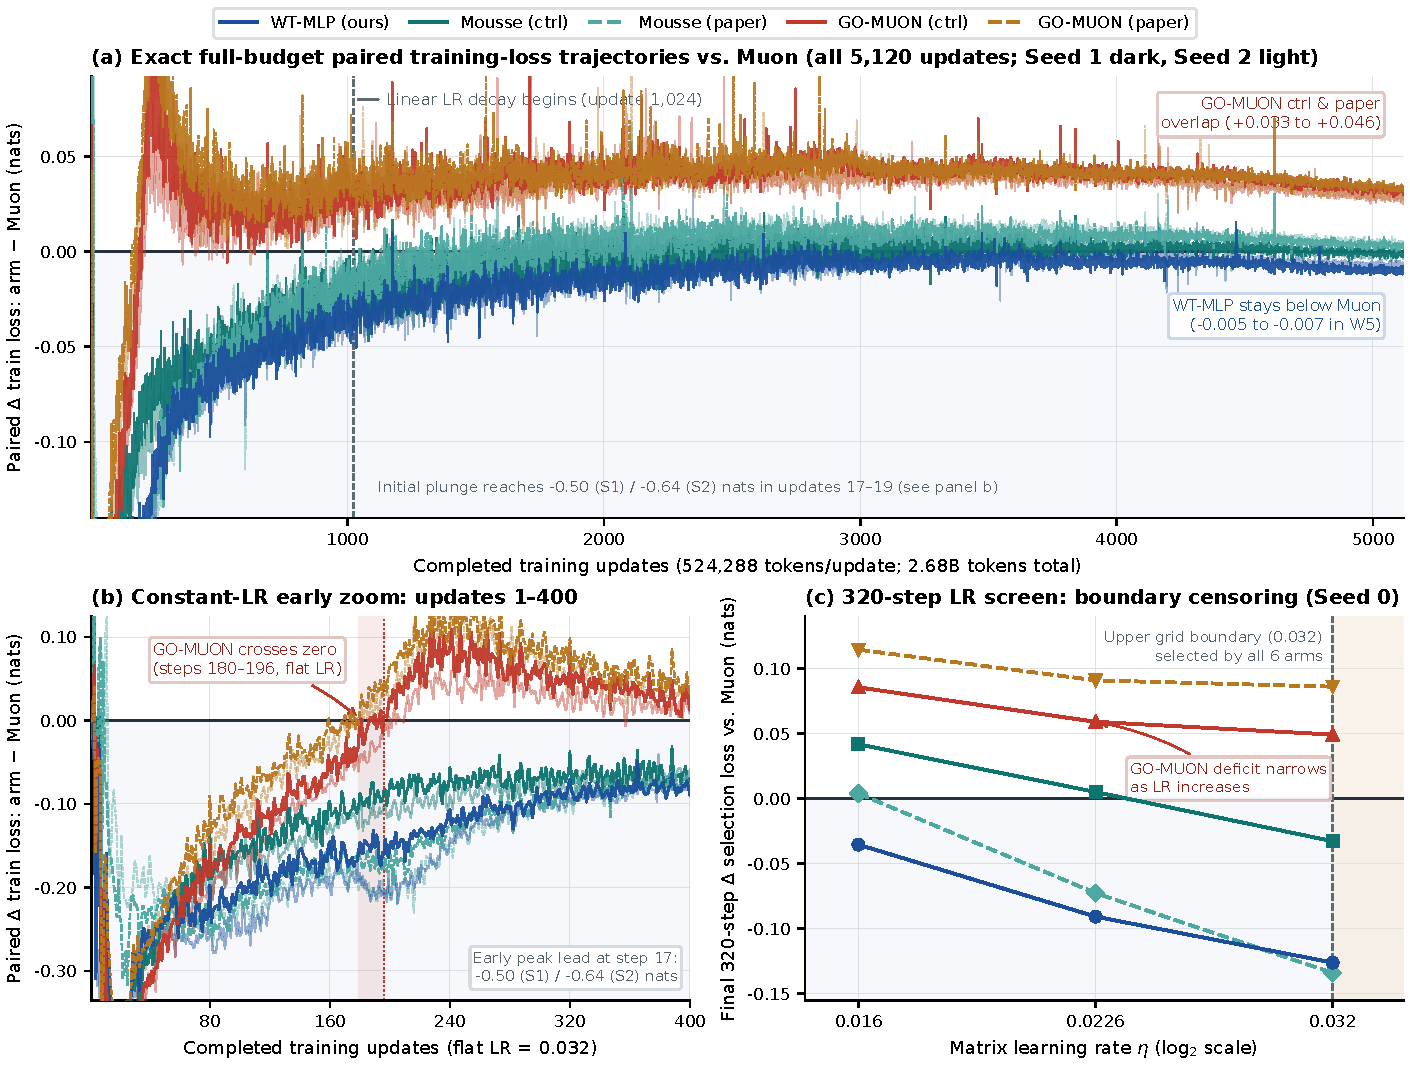
\includegraphics[width=\textwidth]{related_baselines_training.pdf}
\caption{Exact per-update training dynamics and LR-boundary censoring across the
paired related-baseline campaign ($5{,}120$ updates per arm at frozen
$\eta=0.032$ on fresh seeds~1 and~2 under isotropic $\lambda=0.1$ decay; no
smoothing or downsampling).
\textbf{(a)} Paired training-loss difference versus seed-matched
\texttt{muon\_control} (negative favors candidate; Seed~1 darker, Seed~2
lighter).
\textbf{(b)} Early-training zoom (updates $1$--$400$, inside the flat-LR
plateau) showing GO-MUON's initial surge and constant-LR crossover near update
$200$.
\textbf{(c)} 320-update seed-0 LR screen showing monotonic improvement into the
$0.032$ upper grid boundary.}
\label{fig:related}
\end{figure}

\subsection{Q7: Eight-GPU Systems Overhead and Wall-Clock Time-to-Target}
\label{sec:res-q7}

\paragraph{Eliminating barriers, fallback stalls, and SIMT products reduces \texttt{fast\_lag} steady-step overhead to $+3.8\%$--$+5.8\%$ at $130\text{M}$ and $+10.5\%$ at $520\text{M}$.}
On the legacy synchronous research runner, even diagonal-only \taxid{OD-All}
incurred $+10.4\%$ steady-step overhead while \taxid{WT-MLP} paid $+21.9\%$ and
legacy \taxid{WT-MLP-Lag} paid $+18.0\%$. On uncontended eight-A100 nodes,
\texttt{fast\_lag} cuts full-run steady-step overhead over \taxid{MuonT} by more
than $3\times$: to $+\sysExecSymLagVsMuontPct\%$ on \taxid{WT-Sym-Lag}
($\sysExecSymLagGib$\,GiB) and $+\confPTwoWtStepPct\%$--$+\sysExecMlpLagVsMuontPct\%$
on \taxid{WT-MLP-Lag} ($\sysExecMlpLagGib$\,GiB; $+\confPThreeWtStepPct\%$ over
$20{,}480$ steps at $130\text{M}$ $4\times$). At $520\text{M}$ ($d=1024$,
microbatch~1 on 40\,GB A100s), \taxid{WT-MLP-Lag}'s overhead rises modestly to
$+\confPFourWtStepPct\%$ ($\confPFourWtGib{}$ versus $\confPFourMuontGib{}$\,GiB),
remaining well within single-node 40\,GB VRAM.

\paragraph{Bringing step overhead below the $\sysTokenSavingPct\%$ token-saving threshold converts legacy wall-clock deficits into a launch-anchored win at $\text{C4}\le 3.52$.}
At $130\text{M}$ $1\times$, every width-thresholded arm reaches
$\text{C4}\le 3.52$ at update $4{,}501$ ($2.36\text{B}$ tokens) versus update
$4{,}751$ ($2.49\text{B}$ tokens) for \taxid{MuonT} and \taxid{Muon} --- a
$\sysTokenSavingPct\%$ token saving ($250$ updates; Table~\ref{tab:systems-v2}).
Because legacy runners paid $18\%$--$22\%$ per-step overhead, they crossed
targets $600$--$1{,}100$\,s \emph{later} than \taxid{MuonT}. Once
\texttt{fast\_lag} drops overhead to $+\sysExecSymLagVsMuontPct\%$,
\taxid{WT-Sym-Lag} crosses $\text{C4}\le 3.52$ in
$\sysCrossSymLagThreeFiveTwoS$\,s --- ahead of same-wave \taxid{MuonT}
($\sysCrossMuontSymThreeFiveTwoS$\,s), Wave-0 \taxid{MuonT}
($\sysCrossMuontWaveZeroThreeFiveTwoS$\,s), and vanilla \taxid{Muon}
($\sysCrossMuonWaveZeroThreeFiveTwoS$\,s) in launch-anchored wall-clock time,
while \texttt{fast\_lag} \taxid{WT-MLP-Lag} saves $600$\,s over legacy Wave~4
and edges Wave-0 \taxid{MuonT} ($\sysCrossMlpLagFastThreeFiveTwoS$\,s) while
retaining the strongest held-out mixture quality.

\begin{table}[t]
\centering
\caption{Launch-anchored eight-A100 wall-clock time-to-target crossings on
Paloma \texttt{c4\_en} ($130\text{M}$ $1\times$ Chinchilla, seed~0,
$2.68\text{B}$ tokens). Elapsed times include compilation, training,
evaluation, and checkpointing from job launch; step indices mark the first
logged evaluation meeting each C4 threshold. \taxid{Muon} fails to reach
$\text{C4}\le 3.46$ within the $5{,}120$-update budget (censored at
$\waveZeroMuonCfourFinalAbs{}$).}
\label{tab:systems-v2}
\footnotesize\setlength{\tabcolsep}{5.0pt}
\resizebox{\textwidth}{!}{% Generated by scripts/analyze_systems.py. Do not edit.
\begin{tabular}{@{}lrrrrr@{}}
\toprule
Arm (wave / runner) & $\text{C4}\le 3.59$ & $\text{C4}\le 3.52$ & $\text{C4}\le 3.46$ & Final C4 & Total E2E \\
\midrule
\taxid{Muon} {\scriptsize(\texttt{wave0})} & $4{,}880.0$\,s {\scriptsize(step 4{,}251)} & $5{,}467.0$\,s {\scriptsize(step 4{,}751)} & \textcolor{famAbl}{\textbf{Censored}} {\scriptsize($3.4618$)} & $3.4618$ & $5{,}889.7$\,s \\
\taxid{MuonT} {\scriptsize(\texttt{wave0})} & $4{,}721.3$\,s {\scriptsize(step 4{,}001)} & $5{,}566.3$\,s {\scriptsize(step 4{,}751)} & $5{,}848.2$\,s {\scriptsize(step 5{,}001)} & $3.4527$ & $5{,}984.6$\,s \\
\taxid{MuonT} {\scriptsize(\texttt{wave\_sym\_fastlag})} & $4{,}619.6$\,s {\scriptsize(step 4{,}001)} & $5{,}468.4$\,s {\scriptsize(step 4{,}751)} & $5{,}754.4$\,s {\scriptsize(step 5{,}001)} & $3.4511$ & $5{,}891.3$\,s \\
\rowcolor{pagepanel} \textbf{\taxid{WT-Sym-Lag}} {\scriptsize(\texttt{fast\_lag})} & $4{,}869.6$\,s {\scriptsize(step 4{,}001)} & $\mathbf{5{,}458.9}$\,\textbf{s} {\scriptsize(step 4{,}501)} & $6{,}040.3$\,s {\scriptsize(step 5{,}001)} & $\mathbf{3.4482}$ & $6{,}179.3$\,s \\
\rowcolor{pagepanel} \textbf{\taxid{WT-MLP-Lag}} {\scriptsize(\texttt{fast\_lag})} & $4{,}966.4$\,s {\scriptsize(step 4{,}001)} & $5{,}564.6$\,s {\scriptsize(step 4{,}501)} & $6{,}157.2$\,s {\scriptsize(step 5{,}001)} & $3.4491$ & $6{,}300.3$\,s \\
\taxid{WT-Sym} {\scriptsize(no-lag, $\tau=0$)} & $5{,}187.7$\,s {\scriptsize(step 4{,}001)} & $5{,}822.6$\,s {\scriptsize(step 4{,}501)} & $6{,}446.1$\,s {\scriptsize(step 5{,}001)} & $\mathbf{3.4482}$ & $6{,}593.9$\,s \\
\taxid{WT-MLP-Lag} {\scriptsize(legacy Wave 4)} & $5{,}500.6$\,s {\scriptsize(step 4{,}001)} & $6{,}164.4$\,s {\scriptsize(step 4{,}501)} & $6{,}824.2$\,s {\scriptsize(step 5{,}001)} & $\mathbf{3.4480}$ & $6{,}985.7$\,s \\
\taxid{WT-MLP} {\scriptsize(legacy Wave 2)} & $5{,}624.4$\,s {\scriptsize(step 4{,}001)} & $6{,}309.1$\,s {\scriptsize(step 4{,}501)} & $6{,}981.7$\,s {\scriptsize(step 5{,}001)} & $\mathbf{3.4464}$ & $7{,}142.0$\,s \\
\bottomrule
\end{tabular}
}
\end{table}
